\section{Numerical Integration and Solution of Ordinatry Diffential Equations}


\subsection{Problem 7.12}


\begin{figure}[!ht]
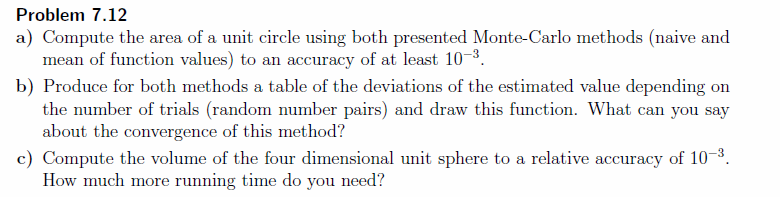
\includegraphics[width=1\textwidth]{chapters/images/desc-7-12}
\end{figure}


X

\begin{lstlisting}[caption=todo]

C

\end{lstlisting}

Y


\subsubsection{a)}

X

\begin{lstlisting}[caption=todo]
def getRandCoord(a, b):
	return random.random() * (b - a) + a;
#

def circleF(x):
	newX = (x % 2) - 1;
	return math.sqrt(1 - pow(newX, 2));
#

def doNaiveMonteCarloTest(xMin, xMax, yMin, yMax):
	randX = getRandCoord(xMin, xMax);
	randY = getRandCoord(yMin, yMax);
	
	return circleF(randX) > randY;
#

goal = math.pi;

def doNaiveMonteCarlo(precision):
	areaEstimated = 0;
	tries = 0.0;
	successes = 0.0;

	while abs(areaEstimated - goal) > precision and tries < 100000:
		if doNaiveMonteCarloTest(0, 4, 0, 1):
			successes += 1;
		
		tries += 1;
		
		areaEstimated = 4 * (successes / tries);
	
	return [areaEstimated, tries];
#

def doMeanMonteCarlo(precision):
	areaEstimated = 0;
	tries = 0.0;
	sum = 0.0;
	
	while abs(areaEstimated - goal) > precision and tries < 100000:
		randX = getRandCoord(0, 4);
		
		sum += circleF(randX);
		tries += 1;
		
		areaEstimated = 4 * (sum / tries);
	
	return [areaEstimated, tries];
#


minError = 0.001;


naiveMonteCarlo = doNaiveMonteCarlo(minError);

print("naive method:");
print("estimated area: " + str(naiveMonteCarlo[0]));
print("tries: " + str(naiveMonteCarlo[1]));

meanMonteCarlo = doMeanMonteCarlo(minError);

print(" ");
print("mean value method:");
print("estimated area: " + str(meanMonteCarlo[0]));
print("tries: " + str(meanMonteCarlo[1]));


\end{lstlisting}


results:

\begin{lstlisting}[caption=Result of 1.1 a), keywordstyle=\color{black}]
naive method:
estimated area: 3.14241702843
tries: 7141.0

mean value method:
estimated area: 3.14239623321
tries: 658.0
\end{lstlisting}

X



\subsubsection{b)}

X

\begin{lstlisting}[caption=todo]

def getNaiveMonteCarloDeviation(tries):
	successes = 0.0;
	
	for i in range(tries):
		if doNaiveMonteCarloTest(0, 4, 0, 1):
			successes += 1;
	
	areaEstimated = 4 * (successes / tries);
	
	return abs(areaEstimated - goal);
#

def getMeanMonteCarloDeviation(tries):
	sum = 0.0;
	
	for i in range(tries):
		randX = getRandCoord(0, 4);
		
		sum += circleF(randX);
	
	areaEstimated = 4 * (sum / tries);
	
	return abs(areaEstimated - goal);
#


xses = [];
naiveYses = [];
meanYses = [];

for i in range(1, 250):
	naiveDeviation = getNaiveMonteCarloDeviation(i * 10);
	meanDeviation = getMeanMonteCarloDeviation(i * 10);
	
	xses.append(i);
	naiveYses.append(naiveDeviation);
	meanYses.append(meanDeviation);


plt.plot(xses, naiveYses);
plt.plot(xses, meanYses);
plt.xlabel("tries");
plt.ylabel("deviation");
plt.show();

\end{lstlisting}


results:


\begin{figure}[!ht]
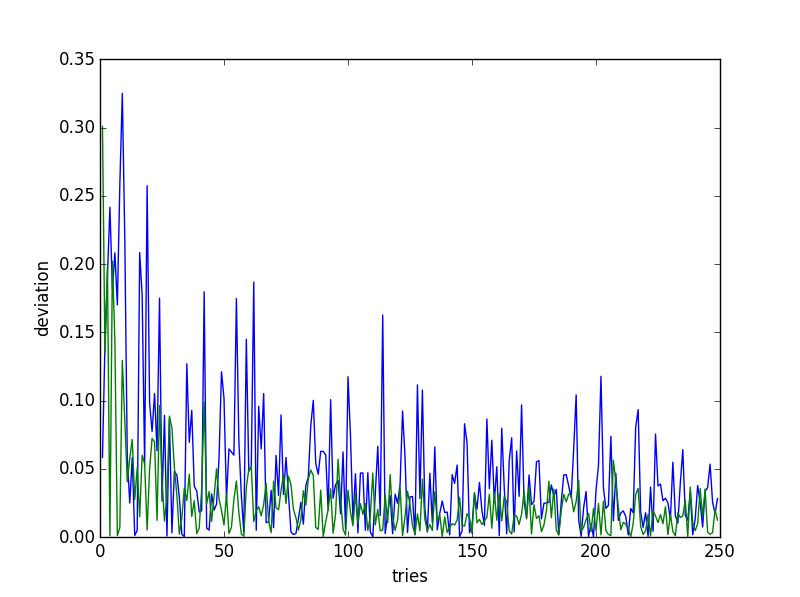
\includegraphics[width=1\textwidth]{chapters/images/figure-7-12-b}
\caption{todo}
\end{figure}


X



\subsubsection{c)}

X

\begin{lstlisting}[caption=todo]
def isIn4DSphere4D(x, y, z, a):
	return math.sqrt(pow(x, 2) + pow(y, 2) + pow(z, 2) + pow(a, 2)) < 1;
#

def doNaiveMonteCarloTest4D():
	randX = getRandCoord(0, 1);
	randY = getRandCoord(0, 1);
	randZ = getRandCoord(0, 1);
	randA = getRandCoord(0, 1);
	
	return isIn4DSphere4D(randX, randY, randZ, randA);
#

goal2 = pow(math.pi, 2) / 2.0;

def doNaiveMonteCarlo4D(precision):
	areaEstimated = 0;
	tries = 0.0;
	successes = 0.0;

	while abs(areaEstimated - goal2) > precision and tries < 1000000:
		if doNaiveMonteCarloTest4D():
			successes += 1;
		
		tries += 1;
		
		areaEstimated = 16 * (successes / tries);
	
	return [areaEstimated, tries];
#



fourDSphere = doNaiveMonteCarlo4D(minError);
print("estimated area of 4D unit sphere: " + str(fourDSphere[0]));

total2DTries = 0.0;
total4DTries = 0.0;

runs = 250;

for i in range(runs):
	total2DTries += doNaiveMonteCarlo(minError)[1];
	total4DTries += doNaiveMonteCarlo4D(minError)[1];

avg2DTries = total2DTries / float(runs);
avg4DTries = total4DTries / float(runs);

print(" ");
print("average tries for 2d unit circle: " + str(avg2DTries));
print("average tries for 4d unit sphere: " + str(avg4DTries));

\end{lstlisting}

The deviation tends to get smaller, yet it doesn't converge.

results:

\begin{lstlisting}[caption=Result of 1.1 a), keywordstyle=\color{black}]
estimated area of 4D unit sphere: 4.93493975904

average tries for 2d unit circle: 4928.92
average tries for 4d unit sphere: 14141.112
\end{lstlisting}

X






\subsection{Problem 7.13}


\begin{figure}[!ht]
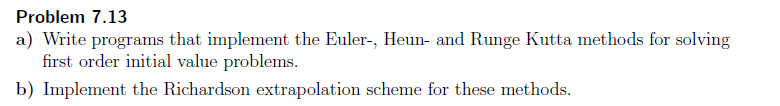
\includegraphics[width=1\textwidth]{chapters/images/desc-7-13}
\end{figure}



\subsubsection{a)}

X

\begin{lstlisting}[caption=todo]

def odeSolver(f, a, b, y0, h, yp1Method):
	yses = [];
	
	x = a;
	y = y0;
	
	yses.append(y);
	
	while x <= b:
		y = yp1Method(f, x, y, h);
		
		yses.append(y);
		
		x += h;
	#
	
	return yses;
#

def eulerYP1(f, x, y, h):
	return y + h * f(x, y);
#

def heunYP1(f, x, y, h):
	k1 = h * f(x, y);
	k2 = h * f(x + h, y + k1);
	
	return y + 0.5 * (k1 + k2);
#

def rungeKuttaYP1(f, x, y, h):
	k1 = h * f(x, y);
	k2 = h * f(x + 0.5 * h, y + 0.5 * k1);
	k3 = h * f(x + 0.5 * h, y + 0.5 * k2);
	k4 = h * f(x + h, y + k3);
	
	return y + (1 / 6.0) * (k1 + 2 * k2 + 2 * k3 + k4);
#


def euler(f, a, b, y0, h):
	return odeSolver(f, a, b, y0, h, eulerYP1);
#

def heun(f, a, b, y0, h):
	return odeSolver(f, a, b, y0, h, heunYP1);
#

def rungeKutta(f, a, b, y0, h):
	return odeSolver(f, a, b, y0, h, rungeKuttaYP1);
#


def odeSystemSolver(fVector, a, b, y0Vector, h, yp1Methods):
	yVectorses = [];
	
	x = a;
	yVector = y0Vector;
	
	yVectorses.append(yVector);
	
	while x <= b:
		yp1Vector = yp1Methods(fVector, x, yVector, h);
		
		yVectorses.append(yp1Vector);
		
		yVector = yp1Vector;
		
		x += h;
	#
	
	return yVectorses;
#

def rungeKuttaYP1System(fVector, x, yVector, h):
	nF = len(fVector);
	
	k1Vector = [];
	yVectorPlusHalfK1Vector = [];
	
	for i in range(nF):
		k1El = h * fVector[i](x, yVector);
		k1Vector.append(k1El);
		yVectorPlusHalfK1Vector.append(yVector[i] + 0.5 * k1El);
	
	k2Vector = [];
	yVectorPlusHalfK2Vector = [];
	
	for i in range(nF):
		k2El = h * fVector[i](x + 0.5 * h, yVectorPlusHalfK1Vector);
		k2Vector.append(k2El);
		yVectorPlusHalfK2Vector.append(yVector[i] + 0.5 * k2El);
	
	k3Vector = [];
	yVectorPlusK3Vector = [];
	
	for i in range(nF):
		k3El = h * fVector[i](x + 0.5 * h, yVectorPlusHalfK2Vector);
		k3Vector.append(k3El);
		yVectorPlusK3Vector.append(yVector[i] + k3El);
	
	yp1Vector = [];
	
	for i in range(nF):
		k4El = h * fVector[i](x + h, yVectorPlusK3Vector);
		
		yp1 = yVector[i] + (1 / 6.0) * (k1Vector[i] + 2 * k2Vector[i] + 2 * k3Vector[i] + k4El);
		
		yp1Vector.append(yp1);
	
	return yp1Vector;
#

def rungeKuttaSystem(fVector, a, b, y0Vector, h):
	return odeSystemSolver(fVector, a, b, y0Vector, h, rungeKuttaYP1System);
#

\end{lstlisting}



X



\subsubsection{b)}

X

\begin{lstlisting}[caption=todo]

def fkFunc(f, x, y, h, yp1Func, q, pk, step):
	if step == 1:
		fh = yp1Func(f, x, y, h);
		fqh = yp1Func(f, x, y, q * h);
	else:
		fh = fkFunc(f, x, y, h, yp1Func, q, pk, step - 1);
		fqh = fkFunc(f, x, y, q * h, yp1Func, q, pk, step - 1);
	
	return fh + ((fh - fqh) / (pow(q, pk) - 1.0));
#

def eulerYP1Richardson(f, x, y, h):
	return fkFunc(f, x, y, h, eulerYP1, 5, 23, 5);
#

def heunYP1Richardson(f, x, y, h):
	return fkFunc(f, x, y, h, heunYP1, 2, 13, 5);
#

def rungeKuttaYP1Richardson(f, x, y, h):
	return fkFunc(f, x, y, h, rungeKuttaYP1, 4, 18, 5);
#

def eulerRichardson(f, a, b, y0, h):
	return odeSolver(f, a, b, y0, h, eulerYP1Richardson);
#

def heunRichardson(f, a, b, y0, h):
	return odeSolver(f, a, b, y0, h, heunYP1Richardson);
#

def rungeKuttaRichardson(f, a, b, y0, h):
	return odeSolver(f, a, b, y0, h, rungeKuttaYP1Richardson);
#


\end{lstlisting}



X

\begin{lstlisting}[caption=todo]

trueVals = [];

for i in range(8): trueVals.append(exT(i / 10.0, 0));

bestError = 9999;
bestQ = -1;
bestPK = -1;

for i in range(2, 6):
	for j in range(2, 25):
		qFU = i;
		pkFU = j;
	
		fns = heunRichardson(exT, 0, 0.6, 1, 0.1);
		
		error = 0;
		
		for k in range(8):
			error += abs(trueVals[k] - fns[k]);
		
		if (error < bestError):
			bestError = error;
			bestQ = qFU;
			bestPK = pkFU;
#

print(bestQ);
print(bestPK);

\end{lstlisting}



X



\subsection{Problem 7.14}


\begin{figure}[!ht]
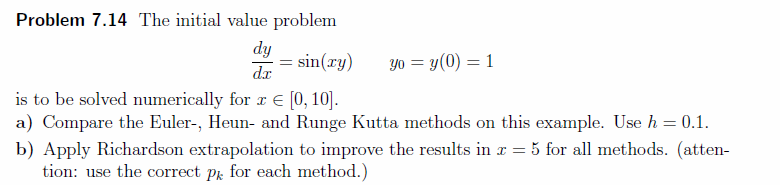
\includegraphics[width=1\textwidth]{chapters/images/desc-7-14}
\end{figure}

(iwo import functions from prob 7.13)

\subsubsection{a)}

X

\begin{lstlisting}[caption=todo]
def myF(x, y):
	return math.sin(x * y);

xses = [];

for i in range(102): xses.append(i / 10.0);

eulerYses = dif.euler(myF, 0, 10, 1, 0.1);
heunYses = dif.heun(myF, 0, 10, 1, 0.1);
rungeKuttaYses = dif.rungeKutta(myF, 0, 10, 1, 0.1);

plt.plot(xses, eulerYses);
plt.plot(xses, heunYses);
plt.plot(xses, rungeKuttaYses);
plt.xlabel("x");
plt.ylabel("y");
plt.show();
\end{lstlisting}


results:

\begin{figure}[!ht]
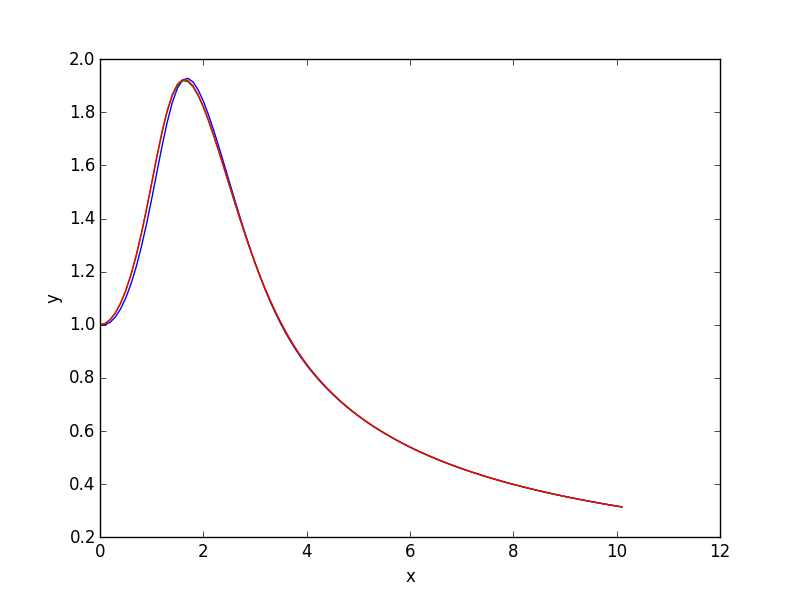
\includegraphics[width=1\textwidth]{chapters/images/figure-7-14-a}
\caption{$\alpha = 2$, initially 3 sheep and 4 wolfs}
\end{figure}



\subsubsection{b)}

X

\begin{lstlisting}[caption=todo]
eulerRichardsonYses = dif.eulerRichardson(myF, 0, 10, 1, 0.1);
heunRichardsonYses = dif.heunRichardson(myF, 0, 10, 1, 0.1);
rungeKuttaRichardsonYses = dif.rungeKuttaRichardson(myF, 0, 10, 1, 0.1);

print("euler: " + str(eulerRichardsonYses[50]));
print("heun: " + str(heunRichardsonYses[50]));
print("runge-kutta: " + str(rungeKuttaRichardsonYses[50]));
\end{lstlisting}


results:

X

\begin{lstlisting}[caption=Result of 1.1 a), keywordstyle=\color{black}]
euler: 0.656662162824
heun: 0.657837825456
runge-kutta: 0.657541150858
\end{lstlisting}

X









\subsection{Problem 7.15}


\begin{figure}[!ht]
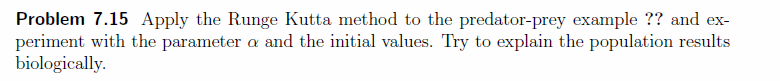
\includegraphics[width=1\textwidth]{chapters/images/desc-7-15}
\end{figure}



X

\begin{lstlisting}[caption=todo]
def sheepFunc10(t, yVector):
	return 10 * yVector[0] * (1 - yVector[1]);
#

def sheepFunc9(t, yVector):
	return 9 * yVector[0] * (1 - yVector[1]);
#

def sheepFunc12(t, yVector):
	return 12 * yVector[0] * (1 - yVector[1]);
#

def wolfsFunc(t, yVector):
	return yVector[1] * (yVector[0] - 1);
#

fses1 = [];
y0ses1 = [];

fses1.append(sheepFunc10);
fses1.append(wolfsFunc);
y0ses1.append(3);
y0ses1.append(1);

fses2 = [];
y0ses2 = [];

fses2.append(sheepFunc9);
fses2.append(wolfsFunc);
y0ses2.append(4);
y0ses2.append(2);

fses3 = [];
y0ses3 = [];

fses3.append(sheepFunc12);
fses3.append(wolfsFunc);
y0ses3.append(3);
y0ses3.append(2);

def testPredatorPrey(fses, y0ses):
	yVectorses = dif.rungeKuttaSystem(fses, 0, 5, y0ses, 0.05);
	
	xses = [];
	sheepYses = [];
	wolfsYses = [];
	
	x = 0;
	
	for yVector in yVectorses:
		sheepYses.append(yVector[0]);
		wolfsYses.append(yVector[1]);
		xses.append(x);
		x += 0.05;
	
	plt.plot(xses, sheepYses);
	plt.plot(xses, wolfsYses);
	plt.xlabel("x");
	plt.ylabel("y");
	plt.show();
#

testPredatorPrey(fses1, y0ses1);
testPredatorPrey(fses2, y0ses2);
testPredatorPrey(fses3, y0ses3);
\end{lstlisting}


results:


\begin{figure}[!ht]
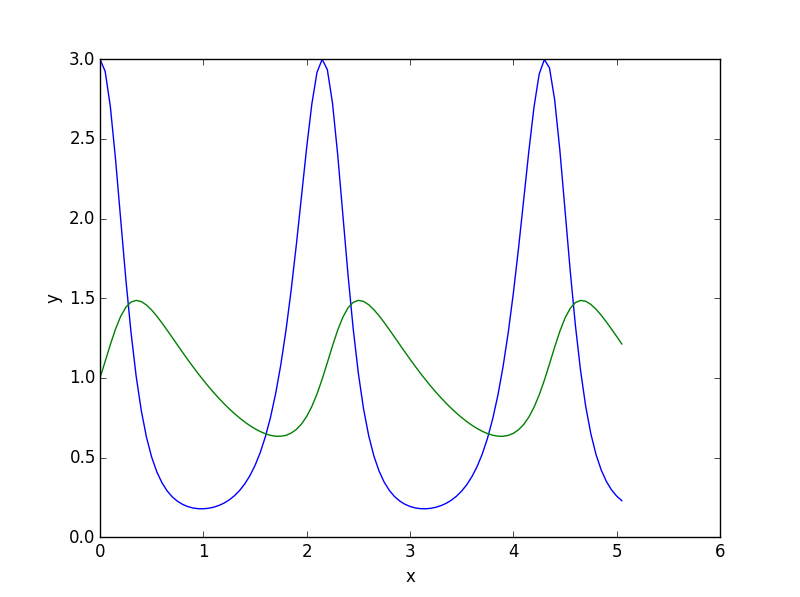
\includegraphics[width=1\textwidth]{chapters/images/figure-7-15-1}
\caption{$\alpha = 2$, initially 3 sheep and 4 wolfs}
\end{figure}


\begin{figure}[!ht]
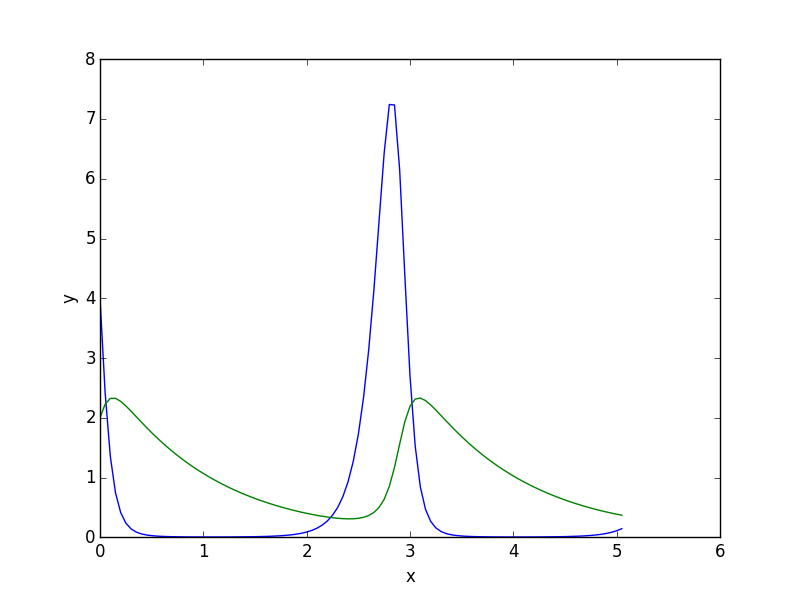
\includegraphics[width=1\textwidth]{chapters/images/figure-7-15-2}
\caption{$\alpha = 2$, initially 3 sheep and 4 wolfs}
\end{figure}


\begin{figure}[!ht]
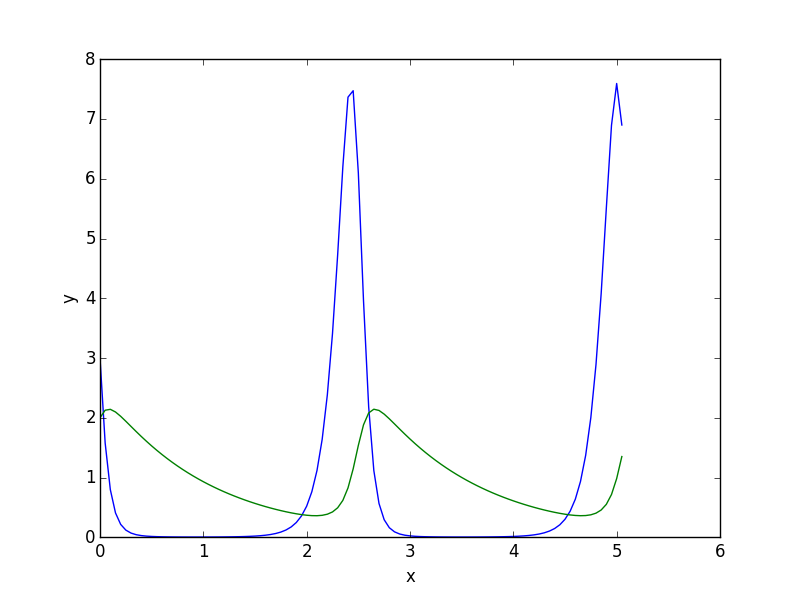
\includegraphics[width=1\textwidth]{chapters/images/figure-7-15-3}
\caption{$\alpha = 2$, initially 3 sheep and 4 wolfs}
\end{figure}







\subsection{Problem 7.16}


\begin{figure}[!ht]
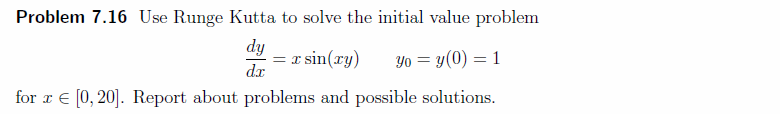
\includegraphics[width=1\textwidth]{chapters/images/desc-7-16}
\end{figure}



X

\begin{lstlisting}[caption=todo]
def myF(x, y):
	return x * math.sin(x * y);
#

xses = [];

for i in range(201): xses.append(i / 10.0);

yses = dif.rungeKutta(myF, 0, 20, 1, 0.1);

plt.plot(xses, yses);
plt.xlabel("x");
plt.ylabel("y");
plt.show();
\end{lstlisting}


results:

\begin{figure}[!ht]
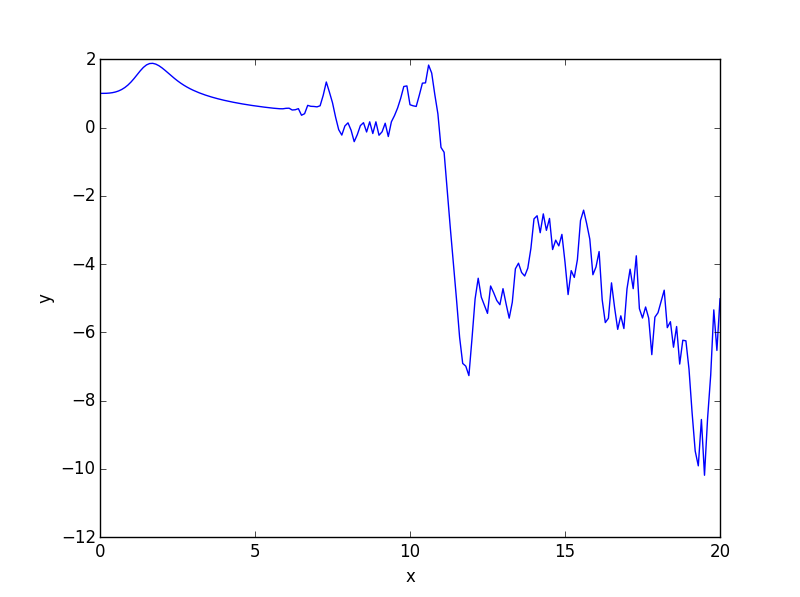
\includegraphics[width=1\textwidth]{chapters/images/figure-7-16}
\caption{$\alpha = 2$, initially 3 sheep and 4 wolfs}
\end{figure}




X


